\documentclass[12pt]{article}

% Setting up the page
\usepackage[margin=20mm,includefoot,footskip=10mm]{geometry}
\usepackage{setspace}
    \onehalfspacing%

% Bibliography, referencing
\usepackage[numbers]{natbib}
    \bibliographystyle{abbrvurl}
\usepackage{hyperref}

% Mathematics, symbols
\usepackage{amssymb}
\usepackage{amsmath}
    \DeclareMathOperator*{\argmin}{arg\,min}
\usepackage{pgf, interval}
    \intervalconfig{soft open fences}

% Images, tables
\usepackage{graphicx}
    \graphicspath{{img/}}
\usepackage{booktabs}
    \renewcommand{\arraystretch}{1.3}
\usepackage{caption}
\usepackage{subcaption}

% Mathematics
\usepackage{amssymb}

% Custom lengths
\newlength{\imgwidth}
\setlength{\imgwidth}{.9\textwidth}
\newlength{\tabwidth}
\setlength{\tabwidth}{.9\textwidth}

\title{%
    Segmentation analysis and the recovery of queuing parameters via the
    Wasserstein distance: a study of administrative data for COPD patients from
    the Cwm Taf region
}
\author{}
\date{}


\begin{document}
\maketitle%

\chapter*{Abstract}
\addcontentsline{toc}{chapter}{Abstract}

This thesis explores three themes related to modern operational research:
evaluating the objective performance of an algorithm, combining clustering with
concepts of mathematical fairness, and developing insightful healthcare models
despite a lack of fine-grained data.

The established evaluation procedure for algorithms --- and particularly machine
learning algorithms --- lacks robustness, potentially inflating the success of
the methods being assessed. To tackle this, the evolutionary dataset
optimisation method is introduced as a supplementary evaluation tool. By
traversing the space in which datasets exist, this method provides the means to
attaining a richer understanding of the algorithm under study.

This method is used to investigate a novel initialisation method for a
centroid-based clustering algorithm, \(k\)-modes. The initialisation makes use
of a matching game to allocate the starting centroids in a mathematically fair
way. The subsequent investigation reveals the conditions under which the new
initialisation improves upon two other initialisation methods.

An extension to the \(k\)-modes algorithm is utilised to segment an
administrative dataset provided by the co-sponsors of this project, the Cwm Taf
Morgannwg University Health Board. The dataset corresponds to the patient
population presenting a specific chronic disease, and comprises a high-level
summary of their stays in hospital over a number of years. Despite the relative
coarseness of this dataset, the segmentation provides a useful profiling of its
instances. These profiles are used to inform a multi-class queuing model
representing a hypothetical ward for the affected patients. Following a novel
validation process for the queuing model, actionable insights into the needs of
the population are found.

In addition to these research pursuits, several open-source software packages
are developed to accompany this thesis. These pieces of software are developed
using best practices to ensure the reliability, reproducibility, and
sustainability of the research in this thesis.

In this section we will conduct a summative and exploratory analysis of the data
provided by the Cwm Taf University Health Board. The focus will be on the
distributions of, and relationships between, our non-trivial cost components
and a selection of other clinical attributes such as length of stay and number
of diagnoses. As we will see in the ensuing analysis, the bulk of this data
corresponds to short-stay and relatively low-cost spells of treatment. Following
this, we will endeavour to construct a framework for the analysis of slices
within the data which provide another dimension to our analysis through
comparison and contrast. However, before any such analysis begins, it is
important to understand the structure of data we are dealing with and how it has
been prepared.

\subsection{Data structure}\label{subsec:structure}

The data is comprised of approximately two and a half million episode-level
records for patients from across Wales that are being treated in the Prince
Charles and Royal Glamorgan hospitals. An episode is defined to be any
continuous period of care provided by the same consultant in the same place. For
instance, if a patient is admitted to a general medical ward for diagnosis and
testing, and then is referred to a specialist consultant in oncology their first
episode would end and be recorded, and a second episode of care would begin on
the oncology ward. Each of these episodes would correspond to a row in the
dataset. If the patient was then discharged, they would have completed a spell
with two episodes. In this analysis we will avoid looking at episode-level
statistics in favour of a patient's spell-level statistics. Since the
introduction of the `payment by results' system for financial flows, it has been
seen that focusing on the more granular episode statistics can lead to the
amount of resource or `activity' consumed by a hospital to treat that patient
being overestimated~\cite{BMJ2004}.

Each episode is recorded as a row of roughly 250 attributes or columns,
including:

\begin{itemize}
    \item Personal identifiers such as identification numbers, age, registered
        GP practice, as well as spell admission and discharge dates;
    \item Other clinical quantities such as the number of diagnoses and
        procedures conducted in that episode, admission and discharge methods,
        and length of stay;
    \item A number of cost components which include the costs coming from
        various departments within the hospital, ward and overhead costs, and
        the cost of administration;
    \item Diagnosis (HRG, ICD10) and procedure (OPCS4) indicators, as well as
        Charlson index scores for a selection of common diagnoses.
\end{itemize}

Of the attributes listed here, we will focus on the cost components and other
clinical variables, paying particular attention to those attributes which are
considered to be linked to overall contribution to the cost of care. Other than
the cost components themselves, those attributes are: true length of stay,
maximum number of diagnoses and total number of procedures in a spell, and the
number of spells associated with any given patient.

\subsection{Cleaning the data}\label{subsec:formatting}

As with many \-- if not all \-- machine learning and knowledge discovery
applications, a substantial amount of preprocessing and formatting was required
to make the data consistent and suitable for our purposes. This process included
the removal of some superfluous columns which added no real information to the
dataset, and a number of rows that had been corrupted by some external storage
software during data collection. In addition to this, we reformatted some
columns whose entries were intended to be used as datetime objects later on.

\section{Constructing the queuing model}\label{sec:model}

Owing to a lack of available data on the system and its patients, the options
for the queuing model used are limited compared to those employed in some modern
works. However, there is a precedent for simplifying healthcare systems to a
single node with parallel servers that emulate resource
availability.~\cite{Steins2013}~and~\cite{Williams2015} provide good examples of
how this approach, when paired with discrete event simulation, can expose the
resource needs of a system beyond deterministic queuing theory models. In
particular,~\cite{Williams2015} shows how a single node, multiple server queue
can be used to accurately predict bed capacity and length of stay distributions
in a critical care unit using administrative data.

Following in the suit of recent literature, a single node using a \(M/M/c\)
queue is employed to model a hypothetical ward of patients presenting COPD.\ In
addition to this, the grouping found in Section~\ref{subsec:overview} provides
a set of patient classes in the queue. Under this model, the following
assumptions are made:
\begin{enumerate}
    \item Inter-arrival and service times of patients are each exponentially
        distributed with some mean. This is in spite of the system time
        distributions shown in Figure~\ref{fig:cluster_los} in order to
        simplify the model parameterisation.
    \item There are \(c \in \mathbb{N}\) servers available to arriving patients
        at the node representing the overall resource availability including bed
        capacity and hospital staff.
    \item There is no queue or system capacity. In~\cite{Williams2015}, a
        queue capacity of zero is set under the assumption that any surplus
        arrivals would be sent to another suitable ward or unit. As this
        hypothetical ward represents COPD patients potentially throughout a
        hospital, this assumption is not held.
    \item Without the availability of expert clinical knowledge, a first-in
        first-out service policy is employed in lieu of some patient priority 
        framework.
\end{enumerate}

Each group of patients has its own arrival distribution. The parameter of this
distribution is taken to be the reciprocal of the mean inter-arrival times for
that group and is denoted by \(\lambda_i\) for each cluster \(i\).

Like arrivals, each group of patients has its own service time distribution.
Without full details of the process order or idle periods during a spell, some
assumption must be made about the true `service' time of a patient in hospital.
It is assumed here that the mean service time of a group of patients may be
approximated via their mean length of stay, i.e.\ the mean time spent in the
system. For simplicity, this work assumes that for each cluster, \(i\), the mean
service time of that cluster, \(\frac{1}{\mu_i}\), to be directly proportional
to the mean total system time of that cluster, \(\frac{1}{\phi_i}\), such that:
\begin{equation}\label{eq:services}
    \mu_i = p_i \phi_i
\end{equation}

\noindent where \(p_i \in \interval[open left]{0}{1}\) is some parameter to be
determined for each group.

One of the few ground truths available in the provided data is the distribution
of the total length of stay. Given that the length of stay and resource
availability are connected, the approach here will be to simulate the length of
stay distribution for a range of values \(p_i\) and \(c\) in order to find the
parameters that best match the observed data.

The statistical comparison of two or more distributions can be done in a number
of ways. Such methods include the Kolmogorov-Smirnov test, a variety of
discrepancy approaches such as summed mean-squared error, and \(f\)-divergences.
A popular choice amongst the latter group (which may be considered
distance-like) is the Kullback-Leibler divergence which measures relative
information entropy from one probability distribution to
another~\cite{Kullback1951}. The key issue with many of these methods is that
they lack interpretability which is paramount when conveying information to
stakeholders. Interpretability not just from explaining how something works but
how its results may be explained also.

As such, a reasonable candidate is the (first) Wasserstein metric, also known as
the `earth mover' or `digger' distance~\cite{Vaserstein1969}. The Wasserstein
metric satisfies the conditions of a formal mathematical metric (like the
typical Euclidean distance), and its values take the units of the distributions
under comparison (in this case: days). Both of these characteristics can aid
understanding and explanation. In simple terms, the distance measures the
approximate `minimal work' required to move between two probability
distributions where `work' can be loosely defined as the product of how much of
the distribution's mass is to be moved and the distance it must be moved
by. More formally, the Wasserstein distance between two probability
distributions \(U\) and \(V\) is defined as:
\begin{equation}\label{eq:wasserstein}
    W(U, V) = \int_{0}^{1} \left\vert F^{-1}(t) - G^{-1}(t) \right\vert dt
\end{equation}

\noindent where \(F\) and \(G\) are the cumulative density functions of \(U\)
and \(V\) respectively. A proof of~\eqref{eq:wasserstein} is presented
in~\cite{Ramdas2017}. The parameter set with the smallest maximum distance
between any cluster's simulated system time distribution and the overall
observed length of stay distribution is then taken to be the most appropriate.

To be specific, let \(T\) denote the system time distribution of all of the
observed data and let \(T_{i,c,p}\) denote the system time distribution for
cluster \(i\) obtained from a simulation with \(c\) servers and
\(p := \left(p_0, p_1, p_2, p_3\right)\). Then the optimal parameter set
\(\left(c^*, p^*\right)\) is given by:
\begin{equation}\label{eq:parameters}
    \left(c^*, p^*\right) = \argmin_{c, p} \left\{%
        \max_{i} \left\{ W\left(T_{i,c,p}, T\right) \right\}%
    \right\}
\end{equation}

The parameter sweep included values of each \(p_i\) from \(0.5\)
to \(1.0\) with a granularity of \(5.0 \times 10^{-2}\) and values of \(c\) from
\(40\) to \(60\) at steps of \(5\).  These choices were informed by the
assumptions of the model and formative analysis to reduce the parameter space
given the computational resources required to conduct the simulations. Each
parameter set was repeated \(50\) times with each simulation running for four
years of virtual time. The warm-up and cool-down periods were taken to be
approximately one year each leaving two years of simulated data from each
repetition.

\begin{figure}
    \centering%
    \begin{subfigure}{.5\imgwidth}
        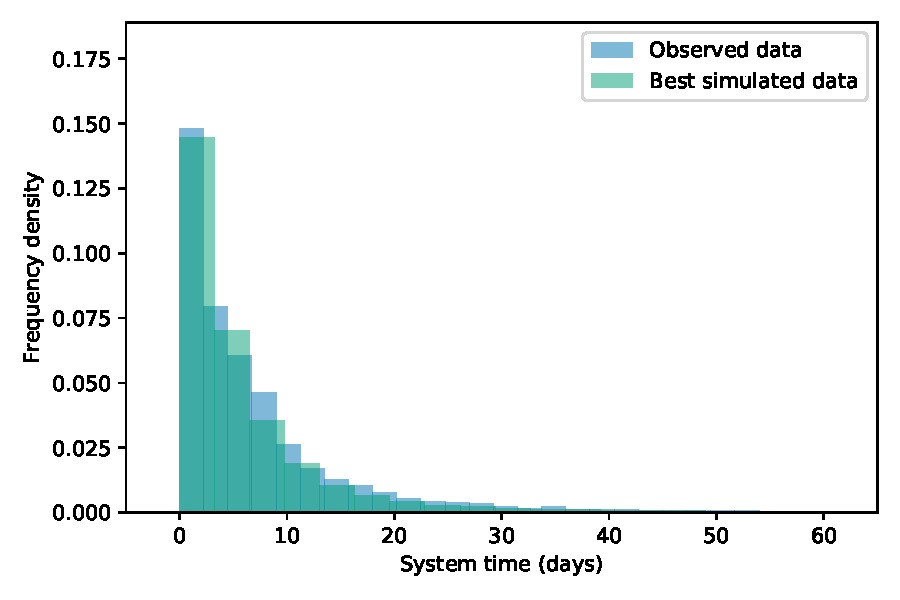
\includegraphics[width=\linewidth]{best_params}
        \caption{}\label{fig:best_params}
    \end{subfigure}\hfill%
    \begin{subfigure}{.5\imgwidth}
        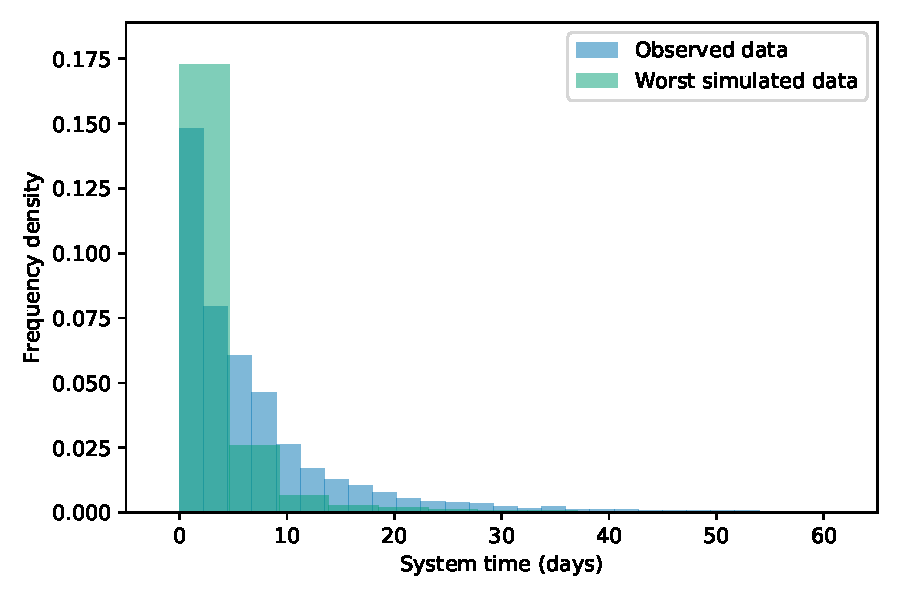
\includegraphics[width=\linewidth]{worst_params}
        \caption{}\label{fig:worst_params}
    \end{subfigure}
    \caption{Histograms of the simulated and observed length of stay data for
             the (\subref{fig:best_params}) best and (\subref{fig:worst_params})
             worst parameter sets.}\label{fig:params}
\end{figure}

The results of this parameter sweep can be summarised in
Figure~\ref{fig:params}. Each plot shows a comparison of the observed lengths
of stay across all groups and the newly simulated data with the best and worst
parameter sets respectively. It can be seen that, in the best case, a very close
fit has been found. Meanwhile, Figure~\ref{fig:worst_params} highlights the
importance of good parameter estimation under this model since the likelihood of
short-stay patient arrivals has been inflated disproportionately against the
tail of the distribution. Table~\ref{tab:comparison} reinforces these results
numerically, showing a clear fit by the best parameters across the board.

\begin{table}
    \centering
    \resizebox{\tabwidth}{!}{\begin{tabular}{lrrrrrrrrrrrrr}
\toprule
{} & \multicolumn{6}{l}{Model parameter and result} & \multicolumn{7}{l}{LOS statistic} \\
{} &                    \(p_0\) & \(p_1\) & \(p_2\) & \(p_3\) & \(c\) & Max. distance &          Mean &   Std. &  Min. &   25\% &  Med. &   75\% &    Max. \\
\midrule
Observed        &                        NaN &     NaN &     NaN &     NaN &   NaN &          0.00 &          7.70 &  11.86 & -0.02 &  1.49 &  4.20 &  8.93 &  224.93 \\
Best simulated  &                       0.95 &     1.0 &     1.0 &     0.5 &  40.0 &          1.28 &          7.00 &  12.09 &  0.00 &  1.44 &  3.57 &  7.65 &  326.46 \\
Worst simulated &                       0.50 &     0.5 &     0.5 &     1.0 &  40.0 &          4.25 &          4.36 &  13.40 &  0.00 &  0.72 &  1.78 &  3.84 &  463.01 \\
\bottomrule
\end{tabular}
}
    \caption{A comparison of the observed data, and the best and worst simulated
        data based on the model parameters and summary statistics for length of
    stay (LOS).}\label{tab:comparison}
\end{table}

In this section, the clustering has been used to enrich the overall queuing
model and to recover the parameters for several classes within that queue to a
high standard. Now, using this model, the next section conducts an investigation
into the underlying system by adjusting the parameters of the queue with the
clustering.

\section{Adjusting the queuing model}\label{sec:scenarios}

This section is comprised of several `what-if' scenarios --- a classic component
of healthcare operational research --- under the novel parameterisation of the
queue established in Section~\ref{sec:model}. The outcomes of interest in this
work are server (resource) utilisation and system times as these metrics capture
the driving forces of cost and flow as well as the overall state of the system,
its staff and its patients. Specifically, the objective of these experiments is
to address the following questions:
\begin{itemize}
    \item How would the system be affected by a change in overall patient
        arrivals?
    \item How is the system affected by a change in resource availability (i.e.\
        a change in \(c\))?
    \item How is the system affected by patients moving between clusters?
\end{itemize}

Owing to the nature of the observed data, the queuing model parameterisation
and its assumptions, the effects on the chosen metrics in each scenario are
given in relative terms with respect to the base case. The base case being those
results generated from the best parameter set recorded in
Table~\ref{tab:comparison}. In particular, the data from each scenario is scaled
by the corresponding median value in the base case meaning that a metric having
a value of 1 is `normal'.

As mentioned in Section~\ref{sec:intro}, the source code used throughout this
work is available online and has been archived. %TODO Add citation for repo
In addition to this, the datasets generated from the simulations in this section
have been archived along with those generated from the parameter
sweep~\cite{Wilde2020results}.


\subsection{Changes to overall patient arrivals}\label{subsec:arrivals}

Changes in overall patient arrivals to a queue reflect real-world scenarios
where some stimulus is improving (or worsening) the condition of the patient
population. Examples of stimuli could include an aging population or
changes to deprivation. Within this model, overall patient arrivals are altered
using a scaling factor denoted by \(\sigma\in\mathbb{R}\). This scaling factor
is applied to the model by multiplying each cluster's arrival rate by
\(\sigma\). That is, for cluster \(i\), its new arrival rate, \(\hat\lambda_i\),
is given by:
\begin{equation}\label{eq:lambda}
    \hat\lambda_{i} = \sigma\lambda_i
\end{equation}

\begin{figure}
    \centering
    \begin{subfigure}{.5\imgwidth}
        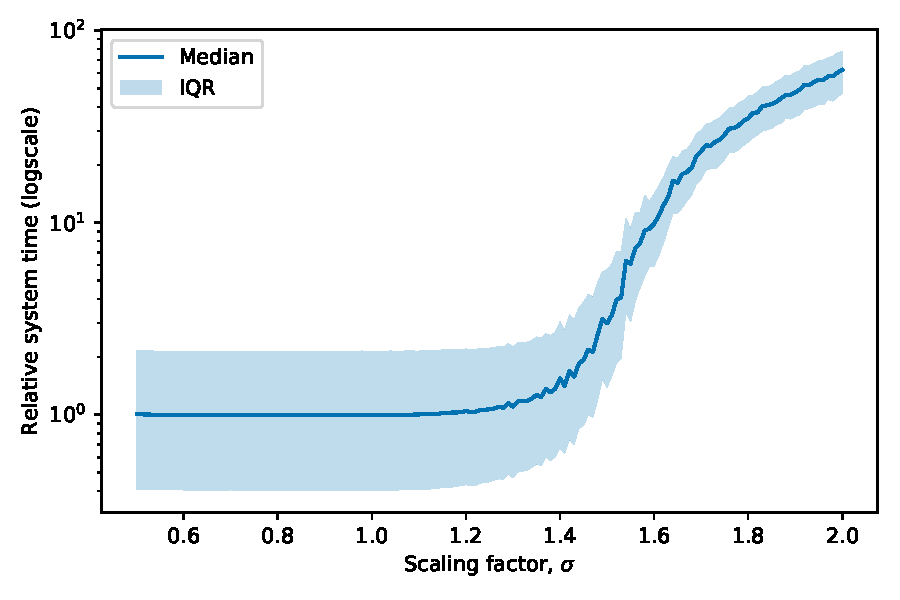
\includegraphics[width=\linewidth]{lambda_time}
        \caption{}\label{fig:lambda_time}
    \end{subfigure}\hfill%
    \begin{subfigure}{.5\imgwidth}
        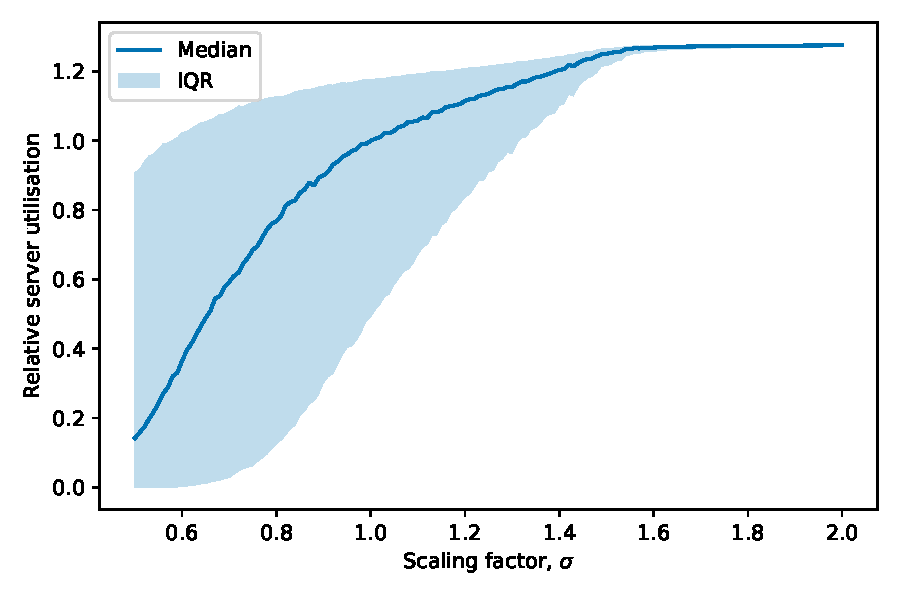
\includegraphics[width=\linewidth]{lambda_util}
        \caption{}\label{fig:lambda_util}
    \end{subfigure}
    \caption{%
        Plots of \(\sigma\) against relative (\subref{fig:lambda_time})~system
        time and (\subref{fig:lambda_util})~server utilisation.
    }\label{fig:lambda}
\end{figure}

Figure~\ref{fig:lambda} shows the effects of changing patient arrivals on
(\subref{fig:lambda_time})~relative system times and
(\subref{fig:lambda_util})~relative server utilisation over values of \(\sigma\)
from 0.5% to 2.0% at a
precision of \(1.0 \times 10^{-2}\)%. Specifically, each plot in the
figure (and the subsequent figures in this section) shows the median and
interquartile range (IQR) of each relative attribute. These metrics provide an
insight into the experience of the average user (or server) in the system, and
in the stability or variation of the body of users (servers).

What is evident from these plots is that things are happening as one might
expect: as arrivals increase, the strain on the system increases. However, it
should be noted that it also appears that the model has some amount of slack
relative to the base case. Looking at Figure~\ref{fig:lambda_time}, for
instance, the relative system times (i.e.\ the relative length of stay for
patients) remains unchanged up to \(\sigma \approx 1.2\), or an approximate 20\%
increase in arrivals of COPD patients. Beyond that, relative system times rise
to an untenable point where the median time becomes orders of magnitude above
the norm.

However, Figure~\ref{fig:lambda_util} shows that the situation for the system's
resources reaches its worst case near to the start of that spike in relative
system times (at \(\sigma \approx 1.4\)). That is, the median server utilisation
reaches a maximum (this corresponds to constant utilisation) at this point and
the variation in server utilisation disappears entirely.


\subsection{Changes to resource availability}\label{subsec:resources}

As is discussed in Section~\ref{sec:model}, the resource availability of the
system is captured by the number of parallel servers in the system, \(c\).
Therefore, to modify the overall resource availability, only the number of
servers need be changed. This kind of sensitivity analysis is usually done to
determine the opportunity cost of adding service capacity to a system, e.g.\
would adding \(n\) servers sufficiently increase efficiency without exceeding
a budget?

To reiterate the beginning of this section, all suitable parameters are given in
relative terms. This includes the number of servers here. By doing this, the
changes in resource availability are more easily seen, and do away with any
concerns as to what a particular number of servers exactly reflects in the real
world.

\begin{figure}
    \centering
    \begin{subfigure}{.5\imgwidth}
        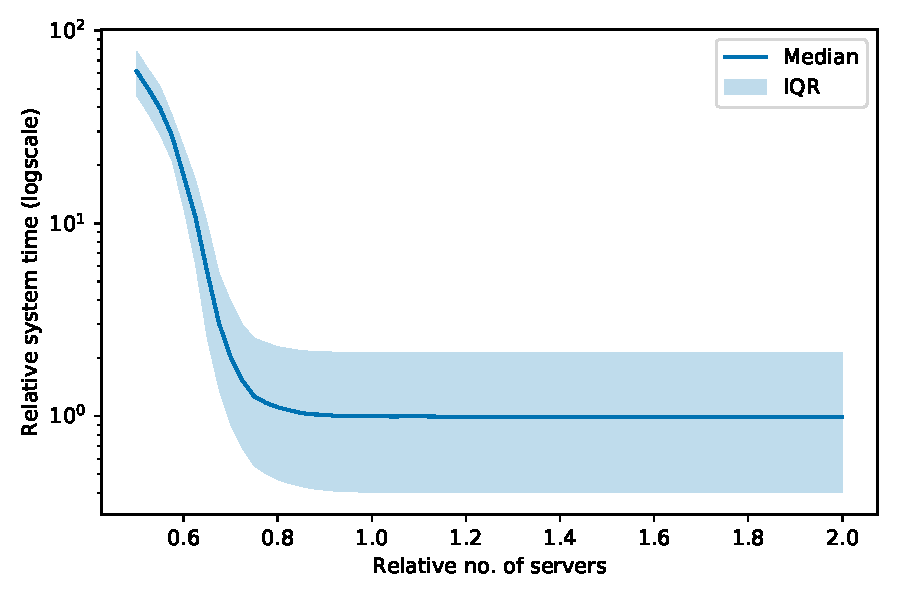
\includegraphics[width=\linewidth]{servers_time}
        \caption{}\label{fig:servers_time}
    \end{subfigure}\hfill%
    \begin{subfigure}{.5\imgwidth}
        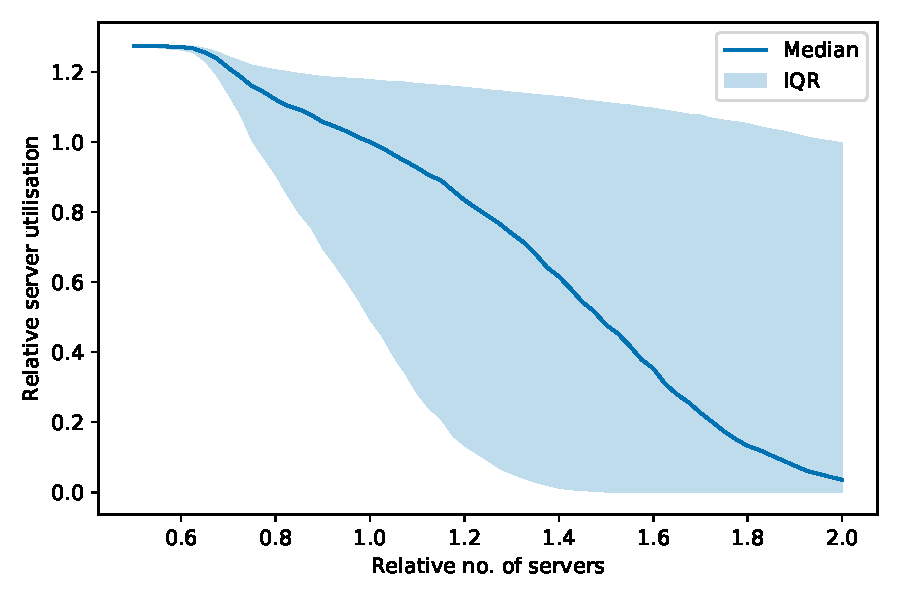
\includegraphics[width=\linewidth]{servers_util}
        \caption{}\label{fig:servers_util}
    \end{subfigure}
    \caption{%
        Plots of the relative number of servers against relative
        (\subref{fig:servers_time})~system time and
        (\subref{fig:servers_util})~server utilisation.
    }\label{fig:servers}
\end{figure}

Figure~\ref{fig:servers} shows how the relative resource availability affects
relative system times and server utilisation. In this scenario, the relative
number of servers took values from 0.5% to
2.0% at steps of
\(2.5 \times 10^{-2}\)% --- this is equivalent to a step size of 1
in the actual number of servers. Overall, these figures fortify the
claim from the previous scenario that there is some room to manoeuvre so that
the system runs `as normal' but pressing on those boundaries results in massive
changes to both resource requirements and system times.

In Figure~\ref{fig:servers_time} this amounts to a maximum of 20\% slack in
resources before relative system times are affected; further reductions quickly
result in a potentially tenfold increase in the median system time, and up to 50
times once resource availability falls by 50\%. Moreover, the variation in the
body of the relative times (i.e.\ the IQR) decreases as resource availability
decreases. The reality of this is that patients arriving at a hospital are
forced to consume larger amounts of resources (simply by being in a hospital)
regardless of their condition, putting added strains on the system.

Meanwhile, it appears that there is no tangible change in relative system times
given an increase in the number of servers. This indicates that the model
carries sufficient resources to cater to the population under normal
circumstances, and that adding service capacity will not necessarily improve
system times.

Again, Figure~\ref{fig:servers_util} shows that there is a substantial change in
the variation in the relative utilisation of the servers. In this case, the
variation dissipates as resource levels fall and increases as they increase.
While the relationship between real hospital resources and the number of servers
is not exact, having variation in server utilisation would suggest that parts of
the system may be configured or partitioned away in the case of some significant
public health event (such as a global pandemic) without overloading the system.


\subsection{Moving arrivals between clusters}\label{subsec:moving}

This scenario is perhaps the most relevant to actionable public health research
of those presented here. The clusters identified in this work could be
characterised by their clinical complexities and resource requirements, as done
in Section~\ref{subsec:overview}. Therefore, being able to model the movement of
some proportion of patient spells from one cluster to another will reveal how
those complexities and requirements affect the system itself. The reality is
then that if some public health policy could be implemented to enact that
movement informed by a model such as this then real change would be seen in the
real system.

In order to model the effects of spells moving between two clusters, the
assumption is that services remain the same (and so does each cluster's \(p_i\))
but their arrival rates are altered according to some transfer proportion.
Consider two clusters indexed at \(i, j\), and their respective arrival rates,
\(\lambda_i, \lambda_j\), and let \(\delta \in [0, 1]\) denote the proportion of
arrivals to be moved from cluster \(i\) to cluster \(j\). Then the new arrival
rates for each cluster, denoted by \(\hat\lambda_i, \hat\lambda_j\)
respectively, are:
\begin{equation}\label{eq:moving}
    \hat\lambda_i = \left(1 - \delta\right) \lambda_i
    \quad \text{and} \quad
    \hat\lambda_j = \delta\lambda_i + \lambda_j
\end{equation}

By moving patient arrivals between clusters in this way, the overall arrivals
are left the same since the sum of the arrival rates is the same. Hence, the
(relative) effect on server utilisation and system time can be measured
independently.

Figures~\ref{fig:moving_time}~and~\ref{fig:moving_util} show the effect of
moving patient arrivals between clusters on relative system time and relative
server utilisation respectively. In each figure, the median and IQR for the
corresponding attribute is shown, as in the previous scenarios. Each scenario
was simulated using values of \(\delta\) from 0.0% to
1.0% at steps of \(2.0 \times 10^{-2}\)%.

Considering Figure~\ref{fig:moving_time}, it is clear that there are some cases
where reducing particular types of spells (by making them like another type of
spell) has no effect on overall system times. Namely, moving the high
resource requirement spells that make up Cluster 0 and Cluster 3 to any other
cluster. These clusters make up only 10\% of all arrivals and this figure shows
that in terms of system times the model is able to handle them without concern
under normal conditions. The concern comes when either of the other clusters
moves to Cluster 0 or Cluster 3. Even as few as one in five of the low
complexity, low resource needs arrivals in Cluster 2 moving to either cluster
results in large jumps in the median system time for all arrivals, and soon
after, as in the previous scenario, any variation in the system times
disappears indicating an overborne system.

With relative server utilisation, the story is much the same. The normal levels
of high complexity, high resource arrivals from Cluster 3 are absorbed by the
system and moving these arrivals to another cluster bears no effect on resource
consumption levels. Likewise, either of the low resource need clusters moving
even slightly toward high resource requirements completely overruns the system's
resources. However, the relative utilisation levels of the system resources can
be reduced by moving arrivals from Cluster 0 to either Cluster 1 or Cluster 2,
i.e.\ by reducing the overall resource requirements of such spells.

In essence, these figures offer two messages: that while some hard spells are
inevitable, they are manageable under the current state of the system, and that
public health policy informed by this model should be preventative in nature. If
an effective policy could be implemented to reduce the resource requirements of
COPD patients when they arrive at a hospital --- for instance, by increasing
access to community care or campaigns against harmful behaviours such as smoking
--- then lengths of stay and strains on the hospital's resources would be
reduced, improving the system as a whole.

\begin{figure}
    \centering
    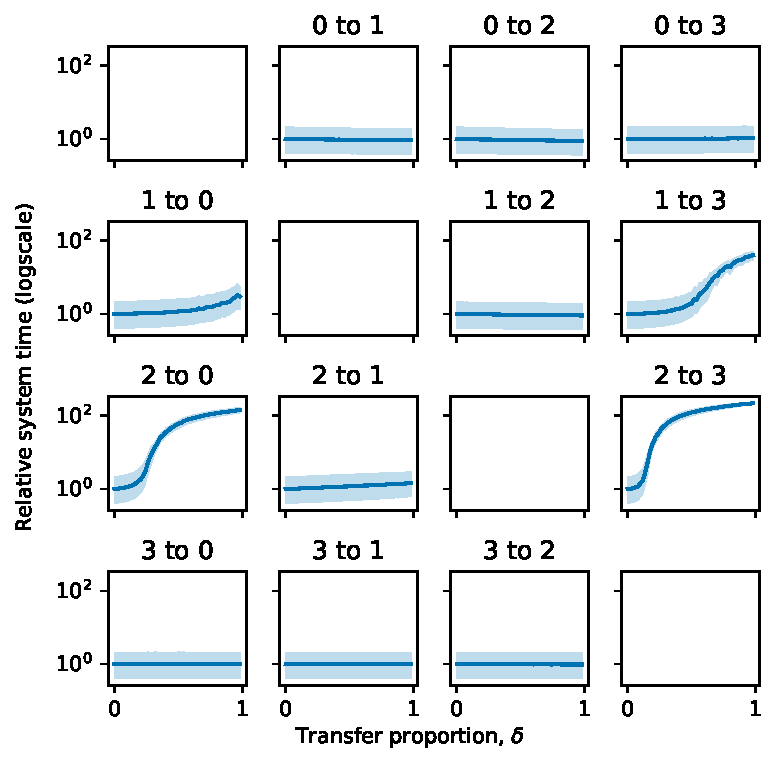
\includegraphics[width=\imgwidth]{moving_time}
    \caption{%
        Plots of proportions of each cluster moving to another against relative
        system time.
    }\label{fig:moving_time}
\end{figure}

\begin{figure}
    \centering
    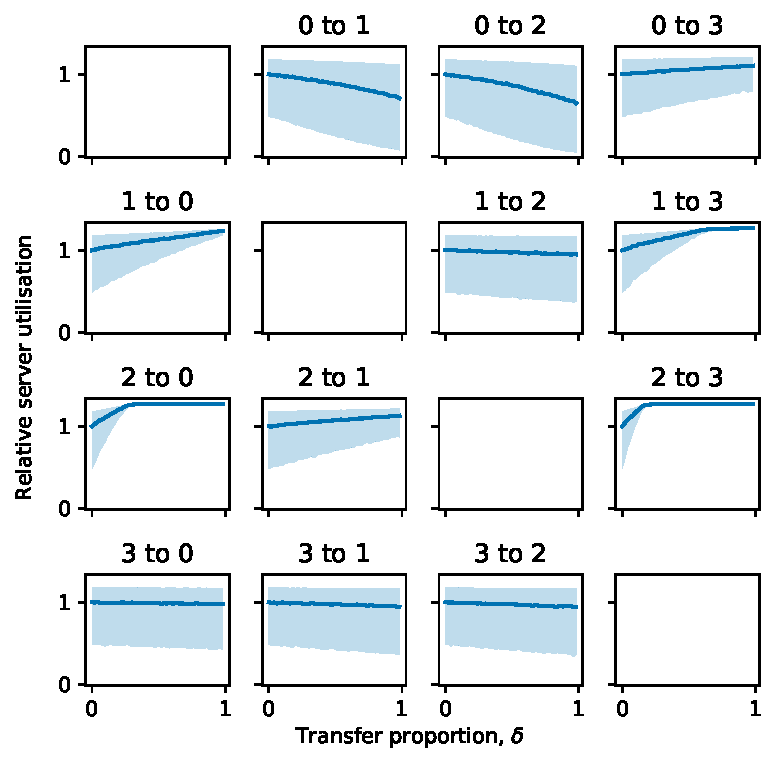
\includegraphics[width=\imgwidth]{moving_util}
    \caption{%
        Plots of proportions of each cluster moving to another on relative
        server utilisation.
    }\label{fig:moving_util}
\end{figure}

\chapter{Conclusions}\label{chp:conc}

This chapter serves to summarise the work reported in this thesis, its
contributions to literature, and potential avenues for further work. Each
chapter in this thesis concluded with a detailed summary, and so the summaries
here are brief.


\section{Research summary}

Chapter~\ref{chp:intro} described the research questions associated with this
thesis, laying out its principle subjects of algorithm evaluation, clustering,
and operational healthcare modelling. With this last subject, there was a
particular interest in overcoming a common issue with machine learning
applications in healthcare: not necessarily having sufficiently detailed and
voluminous data with which to create meaningful, actionable models.

Chapter~\ref{chp:lit} presented a survey of the literature spanning these
principle topics and their intersections. Motivated by the apparent gaps in the
collated literature, the subsequent chapters of the thesis presented novel
methods for assessing the quality of an algorithm (or algorithms), and for
incorporating mathematical fairness into an existing clustering algorithm. These
methods later fed into the case study for \ctmuhb\ which characterised, analysed
and modelled a subsection of their patient population.

In Chapter~\ref{chp:edo}, a new paradigm by which algorithms may be assessed was
described, and a method from that paradigm presented. This method, known as
evolutionary dataset optimisation (EDO), explores the space in which `good'
datasets exist for an algorithm according to some metric. This exploration is
achieved via a bespoke evolutionary algorithm which acts on datasets of unfixed
shapes, sizes and data types. The chapter presented descriptions and
illustrations of the internal mechanisms of the EDO method, as well as briefly
describing a Python implementation. Finally, the chapter concluded with an
extensive case study, demonstrating the capabilities and nuances of EDO in
gaining a richer picture of an algorithm's abilities independently, and against
a competitor.

Following the discussion of `fair' machine learning practices in the literature
review, Chapter~\ref{chp:kmodes} offered a novel initialisation to the
\(k\)-modes algorithm which made use of game theory. The new initialisation
extended a commonly used method, but replaced its greedy component with a
solvable matching game. In the evaluative section of this chapter, traditional
assessment techniques suggested that the new method improved upon the original,
and so the original was discarded.

However, the new method did not consistently outperform another well-known
initialisation. To better understand the conditions under which either of the
remaining initialisations would succeed, a similar competitive setting to
Chapter~\ref{chp:edo} was used. This analysis revealed that there were distinct
sets of properties for which one method was more likely to succeed than the
other according to the metric under study.

Chapter~\ref{chp:copd} presented a novel framework with which to model the
resource needs of a condition-specific healthcare population --- despite a lack
of fine-grained data. In this case, that population were those suffering from
COPD. The corresponding dataset, provided by \ctmuhb, consisted of high-level,
administrative details about the spells associated with the patients, and lacked
the depth that many contemporary operational models require.

The presented framework utilised the clustering algorithm described in
Chapter~\ref{chp:kmodes} to segment a subset of existing and engineered
attributes in the dataset. These attributes included hospital utilisation
metrics, and proxy measures of clinical complexity and resource needs. The
segmentation successfully characterised the instances of the dataset, and the
ensuing analysis of the identified segments revealed clear profiles for each
segment. Included in these profiles were distinctly shaped distributions for
length of stay. With an aim to extract as much as possible from the available
data, and to provide further practical insights, these distributions were
utilised to construct a multi-class queuing model.

The queue, although minimal in structure, produced a well-fitting replica of the
true lengths of stay observed in the data. The quality of this model was
dependent on a novel parameterisation, which derived the unknown service time
distributions for each cluster from the data according to the Wasserstein
distance. In turn, this model was adjusted to answer several `what-if' scenarios
associated with changes in resource capacity and requirements for the population
under study. These adjustments revealed actionable insights into the
most-impactful segments of the population. The most important of these results
was demonstrating the futility of attempting to implement quick, blanket
solutions for that population, such as only increasing resource capacity without
improving patient well-being.


\section{Contributions}\label{sec:contributions}

This thesis has made novel contributions across each of its three principal
themes: algorithm evaluation, clustering, and healthcare modelling. This section
summarises these contributions with reference to their respective chapters.

The EDO method introduced in Chapter~\ref{chp:edo} provided an example approach
from a novel paradigm in which the objective performance of algorithms can be
assessed by exploring the space in which `good' or `bad' datasets exist. The
proposed paradigm expands the commonly used approach for evaluation where a
method's quality is `confirmed' by taking a small number of benchmark datasets
and comparing them with its contemporaries. By exploring the space of datasets,
it was demonstrated that a more robust assessment can be made about a method or
set thereof.

Chapter~\ref{chp:kmodes} added to the growing body of literature where
game-theoretic concepts are combined with machine learning techniques, of which
clustering is included. In general, pursuits of this kind reformulate existing
techniques to be mathematically fair. The initialisation presented in
Chapter~\ref{chp:kmodes}, instead, incorporated game theory directly into an
existing algorithm. In doing so, an improvement over the existing method was
shown, using both traditional confirmation processes and the EDO method.

The framework used in Chapter~\ref{chp:copd} contributed to healthcare modelling
literature in three ways. First, the estimation of queuing parameters via the
Wasserstein distance has expanded a relatively scarce aspect of queuing
research. Second, by making COPD the subject of the methodology, the framework
has added to a body of literature surrounding a condition that is vital to
understand given its prevalence, as well as its links to deprivation and
comorbidity. Lastly, the framework provided a solution to the common issue of
data availability in modern operational research. By combining the various
individual methods, valuable insights were extracted from a relatively
unsophisticated data source, which is a result seldom seen in operational
research.

In addition to the work directly included in the chapters of this thesis, the
research associated with this thesis has resulted in the production of numerous
auxiliary research items. These include several well-developed pieces of
research software, and a number of useful, publicly available datasets for
clustering and healthcare modelling.


\section{Further work}

\subsection*{EDO as a data synthesiser}

As demonstrated in the case study in Chapter~\ref{chp:edo} and the closing
section of Chapter~\ref{chp:kmodes}, the EDO method is capable of facilitating
richer insights into an algorithm's performance. Having said that, a limitation
of the method is that there is no standardised way to guarantee relationships
between different columns in a dataset, \(\mathcal P\), or the families passed
to EDO.  Currently, the only way to do this is to include measures of the
desired relationships in the fitness function. Given the success in the chapters
of this thesis, this level of control is not necessary when looking at an
algorithm (or algorithms) in a general sense, and so is considered beyond the
scope of this thesis.

However, there are cases where automatically ensuring the relationship between
the elements of \(\mathcal P\) could be beneficial to a user of EDO. For
instance, if the algorithm of interest is bespoke to a particular task or
dataset. Using EDO in this way would be analogous to synthesising an existing
dataset, which is another example of when this would be useful. In such a
scenario, it may be beneficial to capture the essence of a dataset by loosely
fitting the elements of \(\mathcal P\) to the existing dataset. Fitting the
parameters of the distribution families would be relatively straightforward, but
incorporating the relationships between them is less so.

This capability has been one of the major attractions of using GANs for data
synthesis, but their black-box nature defeats the object of EDO. Another option
is to use copulas. Copulas are functions that join multivariate distribution
functions to their one-dimensional margins~\cite{Nelsen1999}. For EDO, this
would mean \(\mathcal P\) would contain a single element: a copula function
fitted to the existing dataset. In this case, the technical aspects of an
individual's representation would need adjusting to accommodate this change.
Likewise, the crossover and mutation processes would require some changes to
account for the lack of distinct distribution families.

A Python implementation of copulas for data synthesis exists~\cite{copulas}, and
incorporating this as a dependency of the \edo\ library would reduce the work
required to implement this feature. Studying the impact of copulas in EDO would
provide a valuable opportunity to demonstrate the capabilities of EDO as a fully
fledged data synthesis method.

\subsection*{Expanding the COPD queuing framework}

As discussed at various points in this thesis, the framework presented in
Chapter~\ref{chp:copd} is novel in its ability to circumvent the need for
fine-grained data. However, as discussed in Section~\ref{sec:contributions},
there are other aspects to its novelty. In particular, the use of clustering to
inform a queuing model, and the estimation of unknown queuing parameters.
Extending the reach of this work into the COPD population would be possible with
even slightly more detailed data. For instance, episode-level data (such as the
dataset analysed in Appendix~\ref{app:data}) could allow for a queuing network
with multiple nodes to be developed, separating the various departments in the
hospital. However, that data would need to be well-ordered to understand the
actual pathway of patients at the spell level, which routinely gather
administrative datasets are not.

\ctmuhb, in partnership with Swansea University, have been developing a new
system for recording the clinical activity and vital information of their
patients in real time~\cite{whiteboards}. This system replaces the physical
whiteboards in hospital wards with an electronic equivalent. The `e-whiteboard'
and its drag-and-drop software overcome some of the issues associated with
traditional whiteboards such as the accurate recording of data to the existing
electronic system. In addition, the internal software records the exact time
that information is recorded, allowing for an extremely high level of detail in
terms of the processes undergone by patients. Access to such a data source would
certainly open up more sophisticated models, including both the clustering and
queuing aspects of the framework used in Chapter~\ref{chp:copd}.

\subsection*{Weighted student-project allocation}

In tandem with the work presented in Appendix~\ref{app:biosci}, another School
expressed an interest in implementing a matching-based allocation for their
final year student projects. The attraction of using matching games was the
mathematical fairness of its solution when compared with their current
allocation process. However, their final year students are of two classes: those
on a three-year course and those on a four-year course. Projects for shorter
courses are worth fewer credits and require less commitment from supervisors
than those for longer courses.

Effectively, this variety equates to the students having different weights. A
potential line of research then would be to formulate the weighted
student-project allocation problem (WSA). WSA would be a generalisation of the
student-project allocation problem (SA) --- described in
Appendix~\ref{app:matching} --- where each student, \(s\), would have a weight
associated with them, \(w_s > 0\). Then, the size of a project or supervisor
matching would be the sum of their students' weights, as opposed to the
cardinality of their matching. Under this formulation, an instance of SA could
be restated as an instance of WSA where \(w_s = 1\) for every student, \(s\).

In addition to the formulation, further work would include adapting the existing
Gale-Shapley algorithms for SA to accommodate for student weights, and proving
whether those algorithms guarantee a unique, stable matching.


\bibliography{bibliography}

\end{document}
